\documentclass[11pt]{article}

\makeatletter
%\usepackage{color}
\usepackage{xcolor}
\usepackage{geometry}
%\usepackage[sc]{mathpazo}
\geometry{verbose,tmargin=2.5cm,bmargin=2.5cm,lmargin=2.5cm,rmargin=2.5cm}



\usepackage{setspace}
\usepackage{graphicx, verbatim}  % another package that works for figures
\usepackage{subfigure}  % for subfigures
\usepackage{amsmath}  % for math spacing
%\usepackage{amssymb}  % for math spacing
\usepackage{url}  % Hyphenation of URLs.
\usepackage{lscape}  % Useful for wide tables or figures.
\usepackage[justification=raggedright]{caption}	% makes captions ragged right - thanks to Bryce Lobdell
\usepackage{times}  %change font to times new roman!! take that computer modern!
\usepackage{pgfgantt}
\usepackage{fancyvrb}  %customize commands for typesets
\DefineShortVerb{\|}   %customized |..| to type inline code font

\setlength{\textwidth}{6.5in} 
\setlength{\textheight}{9in}
\setlength{\oddsidemargin}{0in} 
\setlength{\evensidemargin}{0in}
\setlength{\topmargin}{-1.5cm}




\title{Hypothesis/Results}
\date{March 29, 2013}
\author{safyre}

\begin{document}






\maketitle

\section{Baseline Data}

The objective of this section is to characterize the nematode and soybean populations without virus infection.  The |zero_inf| or \emph{zero infection} simulation run constitutes the project's control experiment.



%After connecting to the database, we can extract a table and run statistics on %the data it contains.



%First, however, we'll create a sub table with data that have time references. (hidden)

\begin{knitrout}
\definecolor{shadecolor}{rgb}{0.969, 0.969, 0.969}\color{fgcolor}\begin{kframe}
\begin{alltt}
zinf_sub <- \hlfunctioncall{subset}(zeroinf, NemDiff != 0 & NemDiff > 
    -40000)
zinf_sub <- \hlfunctioncall{subset}(zinf_sub, Tick != 0)
zinf_sub$yr <- zinf_sub$Tick%/%365
\end{alltt}
\end{kframe}
\end{knitrout}



\begin{figure}
\begin{knitrout}
\definecolor{shadecolor}{rgb}{0.969, 0.969, 0.969}\color{fgcolor}\begin{kframe}
\begin{alltt}
\hlfunctioncall{hist}(zinf_sub$NemDiff/zinf_sub$Nematodes, prob = T, breaks = 30, 
    xlab = \hlstring{"Nematode Distribution"}, col = \hlstring{"light blue"}, 
    xlim = \hlfunctioncall{c}(-0.5, 0.5), ylim = \hlfunctioncall{c}(0, 50), main = \hlstring{""})
\hlfunctioncall{lines}(\hlfunctioncall{density}(zinf_sub$NemDiff/zinf_sub$Nematodes), lwd = 2)

\hlfunctioncall{for} (year in \hlfunctioncall{unique}(zinf_sub$yr)) \{
    year_sub <- \hlfunctioncall{subset}(zinf_sub, yr == year)
    \hlfunctioncall{lines}(\hlfunctioncall{density}(year_sub$NemDiff/year_sub$Nematodes), 
        col = \hlfunctioncall{rainbow}((year + 1)/10.1))
    
\}
\end{alltt}
\end{kframe}

{\centering 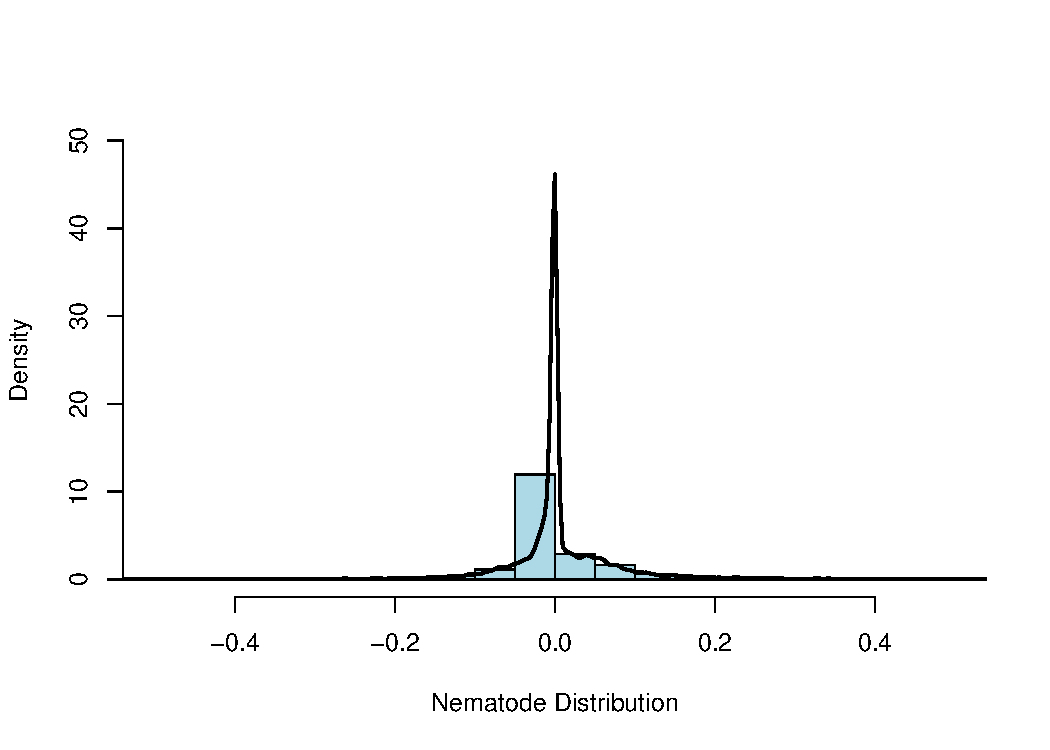
\includegraphics{figure/hist1} 

}



\end{knitrout}

\caption[histogram1]{Histogram of Nemaotode Distrubution without virus infection}
\end{figure}

\begin{figure}
\begin{knitrout}
\definecolor{shadecolor}{rgb}{0.969, 0.969, 0.969}\color{fgcolor}\begin{kframe}
\begin{alltt}
\hlfunctioncall{hist}(zinf_sub$Health_mean, prob=T, breaks=30, xlab = \hlstring{'Mean Nematode Health'},
 col=\hlstring{"light blue"},xlim = \hlfunctioncall{c}(40, 100), ylim= \hlfunctioncall{c}(0, 0.05), main = \hlstring{""})
\hlfunctioncall{lines}(\hlfunctioncall{density}(zinf_sub$Health_mean), lwd=2)

\hlfunctioncall{for}(year in \hlfunctioncall{unique}(zinf_sub$yr)) \{
	year_sub <- \hlfunctioncall{subset}(zinf_sub, yr==year)
	\hlfunctioncall{lines}(\hlfunctioncall{density}(year_sub$Health_mean), col=\hlfunctioncall{gray}((year+1)/10.1))
\}
\end{alltt}
\end{kframe}

{\centering 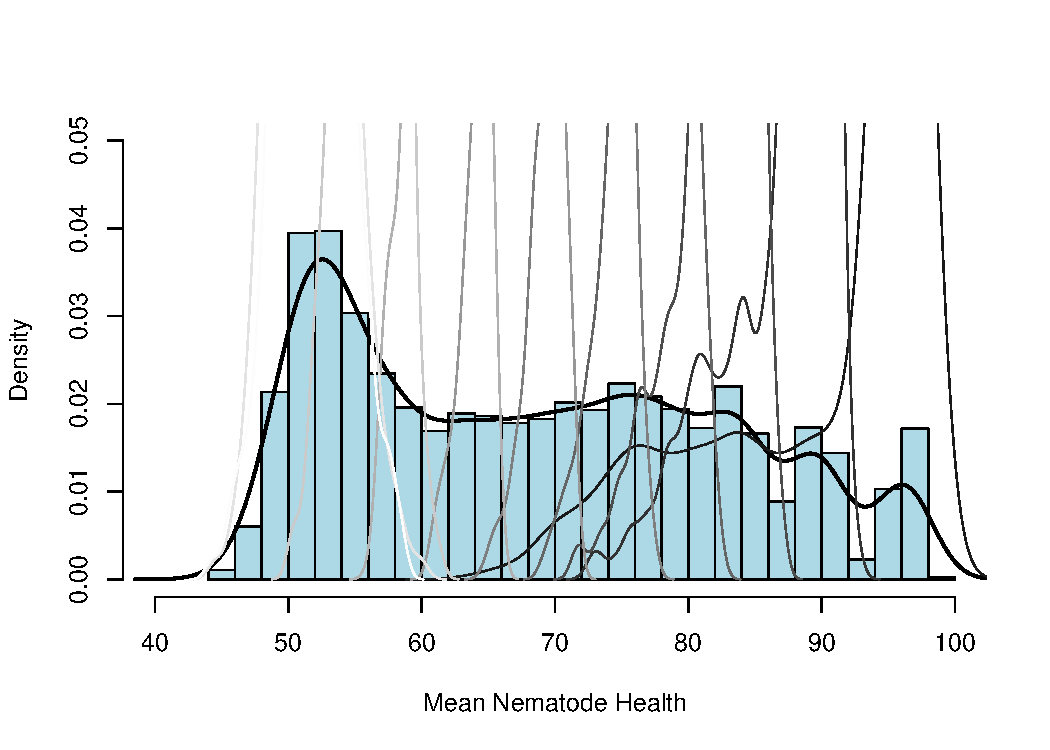
\includegraphics{figure/hist2} 

}



\end{knitrout}

 \caption{Mean Health without Virus infection}
 \end{figure}
 
\begin{figure}
\begin{knitrout}
\definecolor{shadecolor}{rgb}{0.969, 0.969, 0.969}\color{fgcolor}\begin{kframe}
\begin{alltt}
\hlfunctioncall{boxplot}(NemDiff/Nematodes ~ yr, zinf_sub, pch = \hlstring{"."}, 
    main = \hlstring{"Nematode inhibition by year"}, xlab = \hlstring{"Year"}, 
    ylab = \hlstring{"Inhibition"})
\end{alltt}
\end{kframe}

{\centering 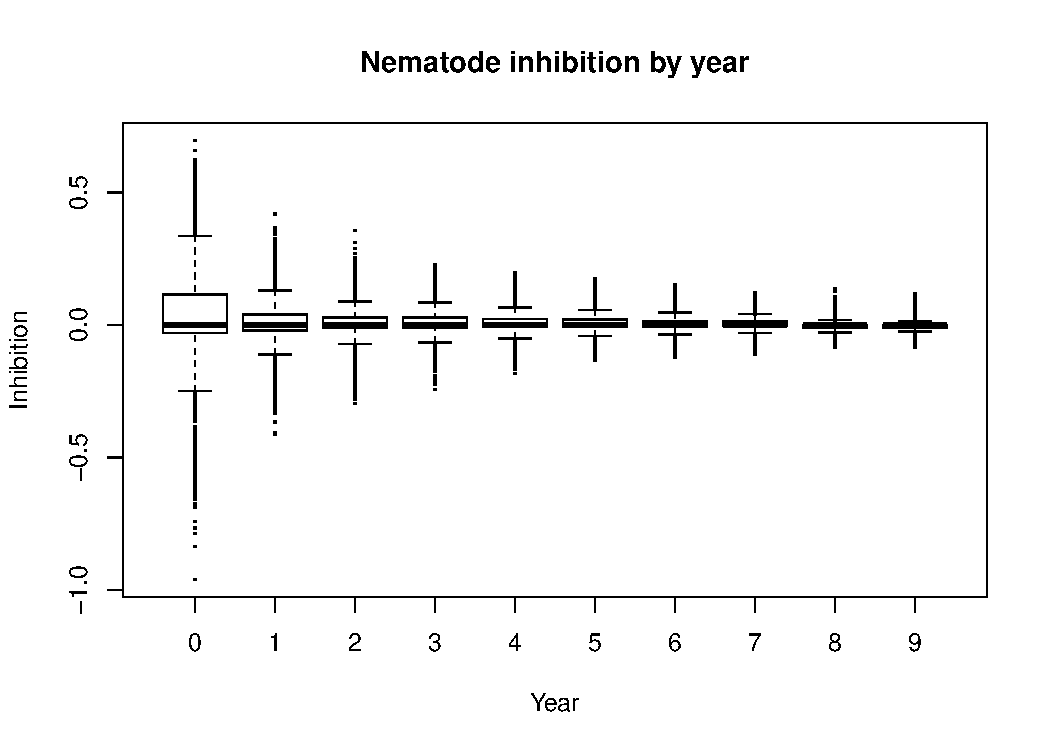
\includegraphics{figure/box1} 

}



\end{knitrout}

\caption[boxplot1]{Nematode distrubution??}
\end{figure}


Boxes 2 and 3 should show up below here.
\begin{knitrout}
\definecolor{shadecolor}{rgb}{0.969, 0.969, 0.969}\color{fgcolor}\begin{kframe}
\begin{alltt}
box2 <- \hlfunctioncall{boxplot}(Health_mean ~ yr, zinf_sub, pch=\hlstring{"."},                
	main=\hlstring{"Mean Nematode Health by year"}, 
	xlab=\hlstring{"Year"}, ylab=\hlstring{"\hlfunctioncall{Health} (%)"});

box3 <-\hlfunctioncall{boxplot}(Health_stdev ~ yr, zinf_sub, pch=\hlstring{"."},
	main=\hlstring{"Mean Nematode Health by year"}, 
	xlab=\hlstring{"Year"}, ylab=\hlstring{"\hlfunctioncall{Health} (%)"});
\end{alltt}
\end{kframe}

{\centering 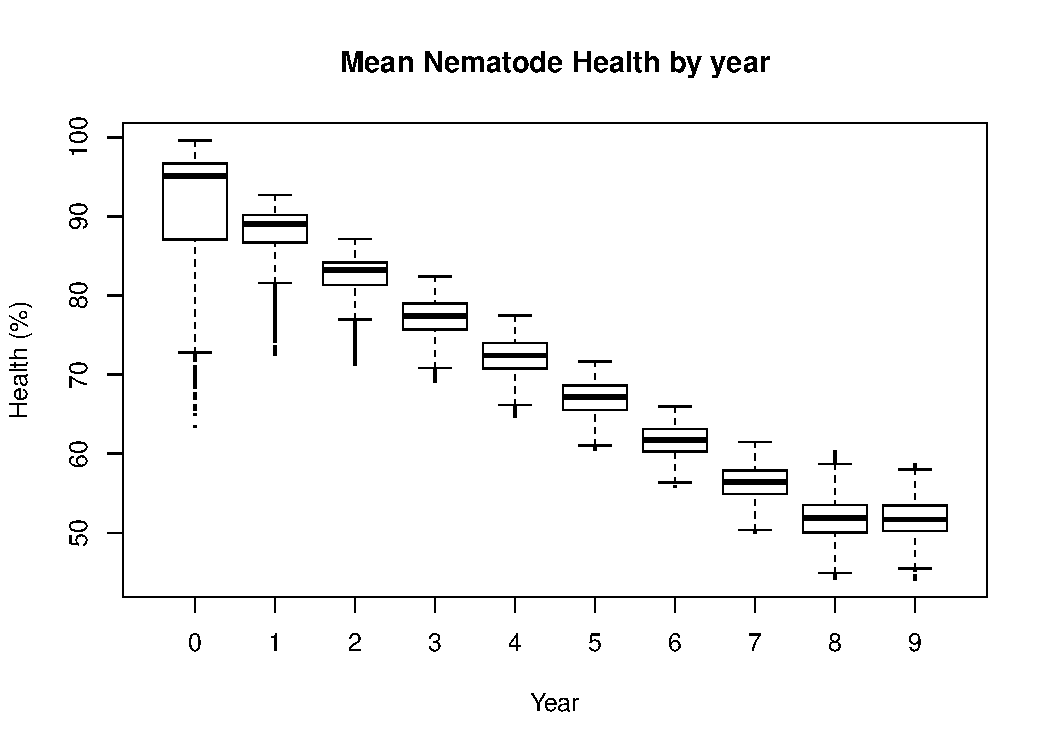
\includegraphics{figure/box2-31} 
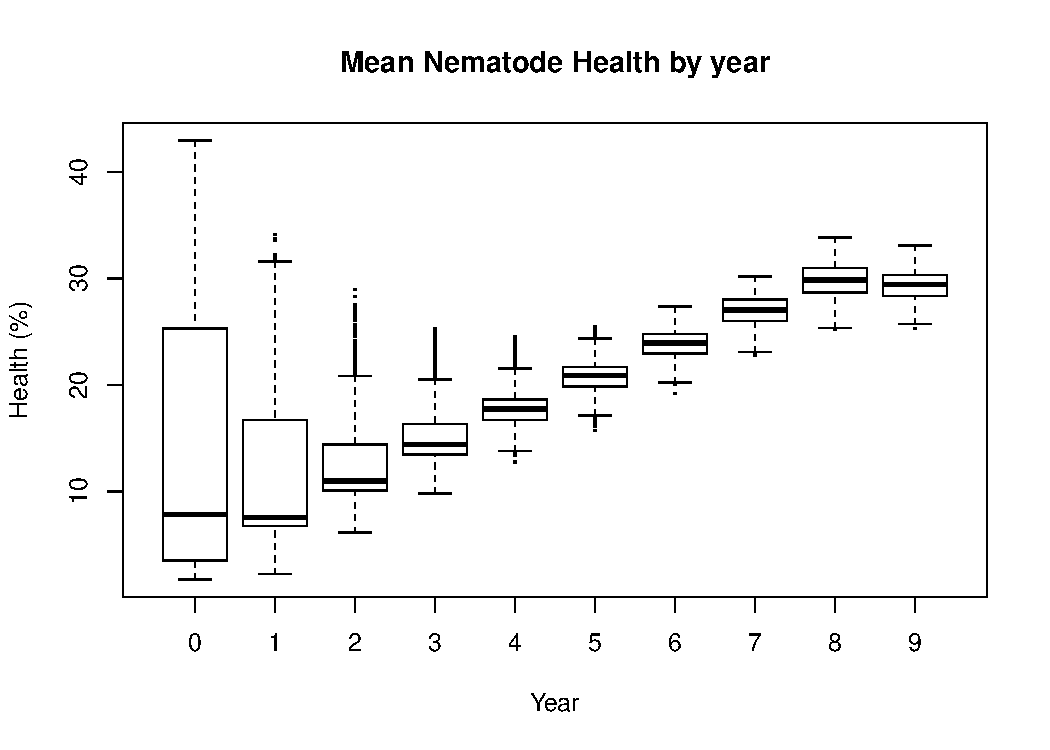
\includegraphics{figure/box2-32} 

}



\end{knitrout}


Looks like issue is above somehow.\\  Coplot is below
\begin{knitrout}
\definecolor{shadecolor}{rgb}{0.969, 0.969, 0.969}\color{fgcolor}\begin{kframe}
\begin{alltt}
\hlfunctioncall{coplot}(Health_stdev ~ Health_mean | yr, zinf_sub, pch = \hlstring{"."}, 
    rows = 1)
\end{alltt}
\end{kframe}

{\centering 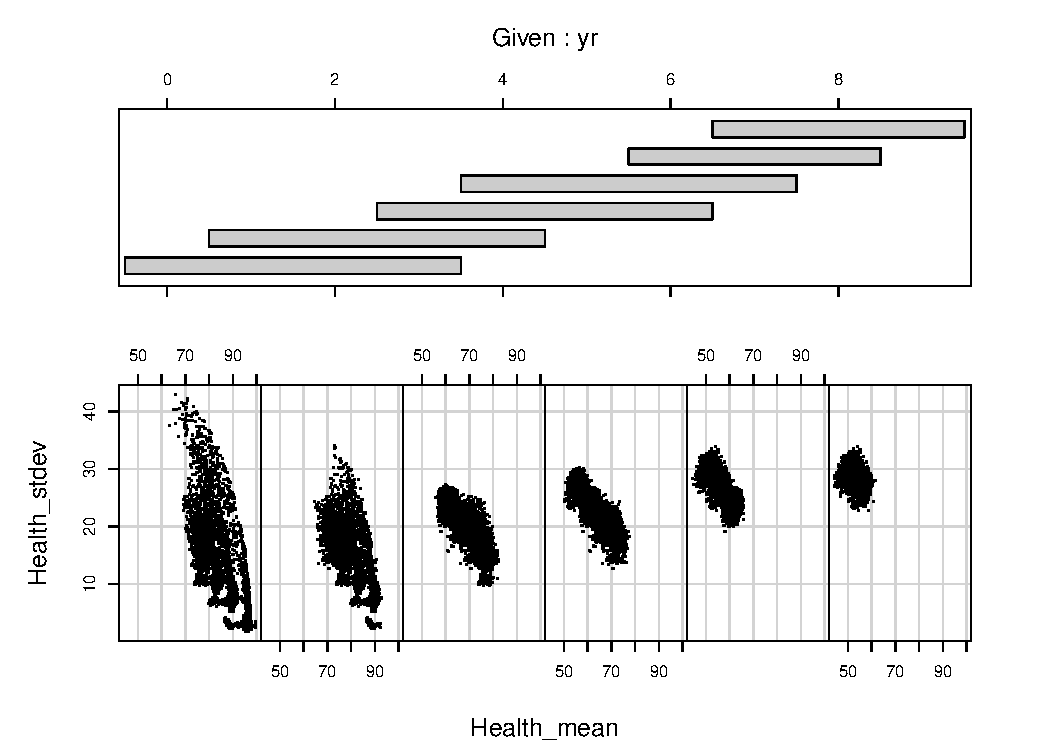
\includegraphics{figure/co-plot} 

}



\end{knitrout}




\begin{knitrout}
\definecolor{shadecolor}{rgb}{0.969, 0.969, 0.969}\color{fgcolor}\begin{kframe}
\begin{alltt}
\hlfunctioncall{boxplot}(NemDiff/Nematodes ~ yr, zinf_sub, pch=\hlstring{"."},
	at = 0:4 - 0.2, boxwex=0.25, col=\hlstring{"lightblue"},
	subset = yr <= 4, 
	main=\hlstring{"Nematode inhibition by year"}, 
	xlab=\hlstring{"Year"}, ylab=\hlstring{"Inhibition"})
       
\hlfunctioncall{boxplot}(Health_mean ~ yr, zinf_sub, pch=\hlstring{"."},
	at = 0:4 - 0.2, boxwex=0.25, col=\hlstring{"lightblue"},
	subset = yr <= 4, 
	main=\hlstring{"Mean Nematode Health by year"}, 
	xlab=\hlstring{"Year"}, ylab=\hlstring{"\hlfunctioncall{Health} (%)"})
	
\end{alltt}
\end{kframe}

{\centering 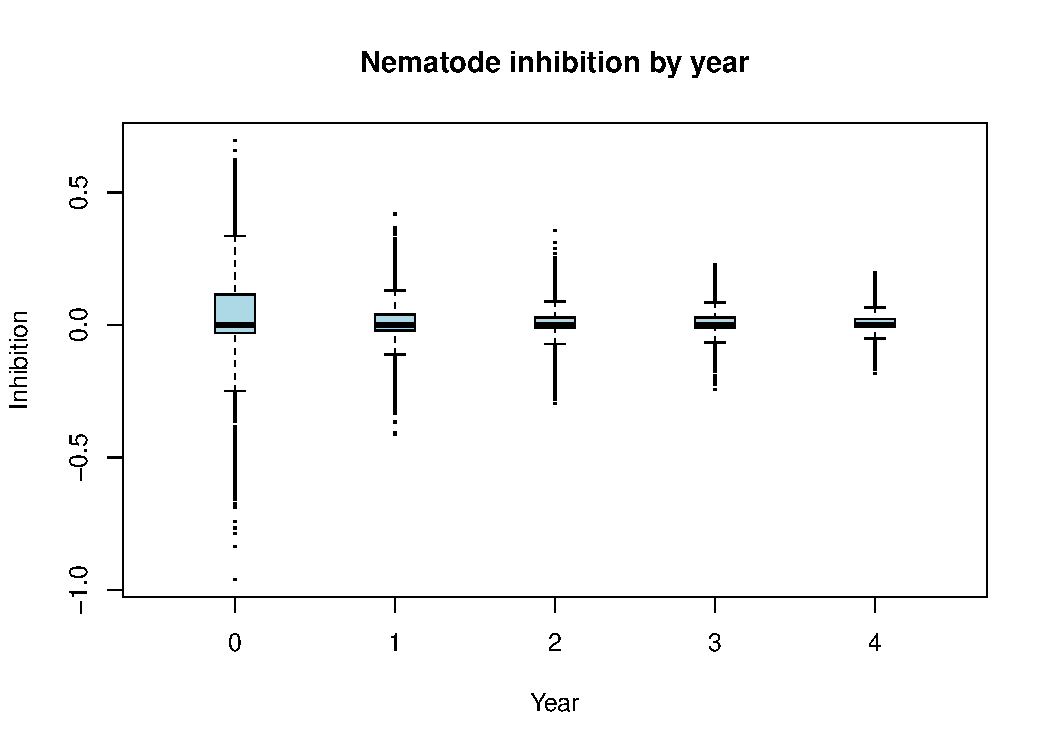
\includegraphics{figure/box-rest1} 
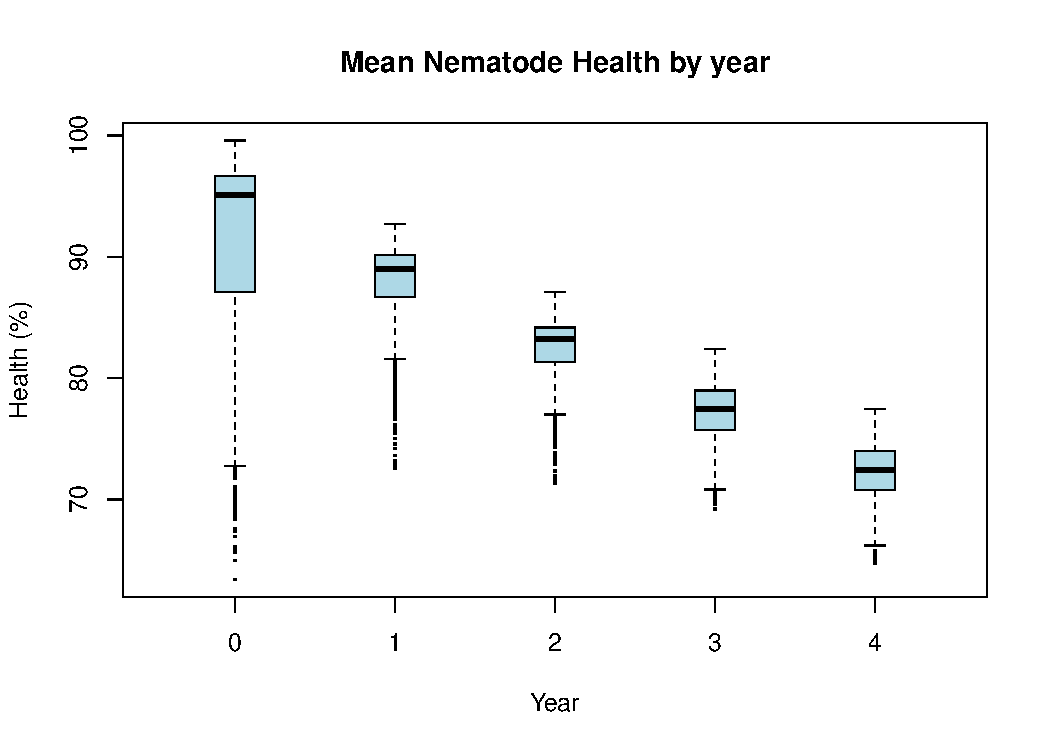
\includegraphics{figure/box-rest2} 

}



\end{knitrout}


More plots...let's see 

\begin{knitrout}
\definecolor{shadecolor}{rgb}{0.969, 0.969, 0.969}\color{fgcolor}\begin{kframe}
\begin{alltt}
\hlfunctioncall{boxplot}(NemDiff/Nematodes ~ yr, zinf_sub, pch=\hlstring{"."},
	at = 0:4 - 0.2, boxwex=0.25, col=\hlstring{"lightblue"},
	subset = yr <= 4, 
	main=\hlstring{"Nematode inhibition by year"}, 
	xlab=\hlstring{"Year"}, ylab=\hlstring{"Inhibition"})
	
\hlfunctioncall{legend}(\hlstring{"bottomright"}, \hlfunctioncall{c}(\hlstring{"No viruses"}),
       fill = \hlfunctioncall{c}(\hlstring{"lightblue"}))
       
\hlfunctioncall{boxplot}(Health_mean ~ yr, zinf_sub, pch=\hlstring{"."},
	at = 0:4 - 0.2, boxwex=0.25, col=\hlstring{"lightblue"},
	subset = yr <= 4, 
	main=\hlstring{"Mean Nematode Health by year"}, 
	xlab=\hlstring{"Year"}, ylab=\hlstring{"\hlfunctioncall{Health} (%)"})
	
\hlfunctioncall{boxplot}(Nematodes ~ yr, zinf_sub, pch=\hlstring{"."},
	at = 0:4 - 0.2, boxwex=0.25, col=\hlstring{"lightblue"},
	subset = yr <= 4, 
	main=\hlstring{"Nematode inhibition by year"}, 
	xlab=\hlstring{"Year"}, ylab=\hlstring{"Inhibition"})
\end{alltt}
\end{kframe}

{\centering 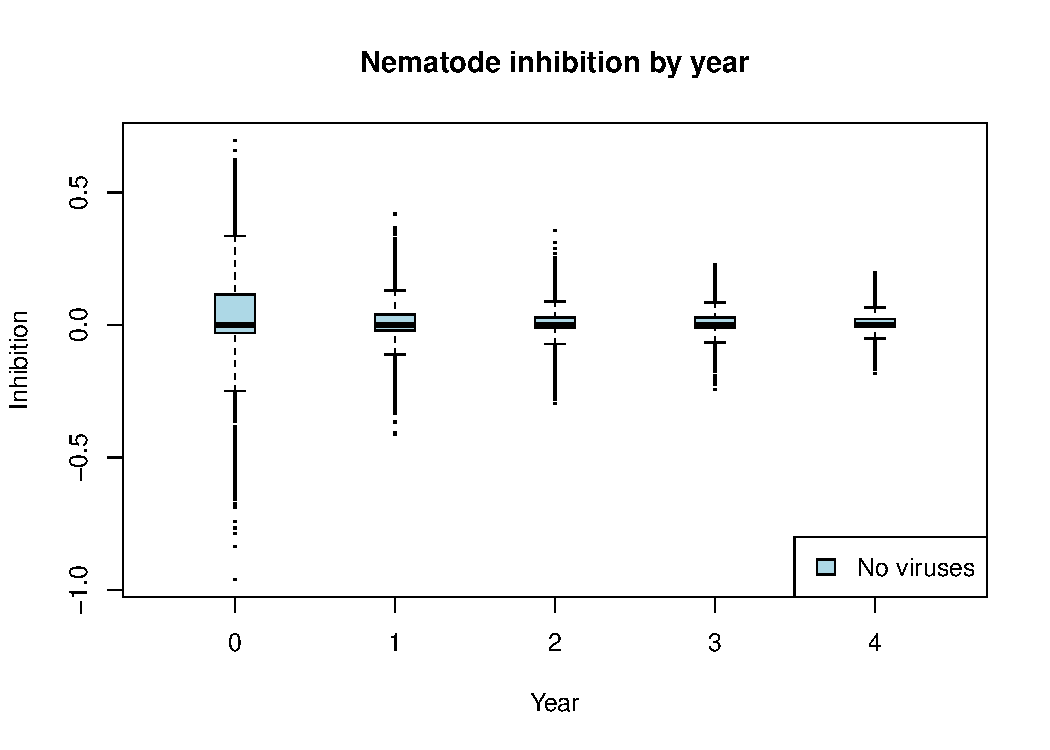
\includegraphics{figure/box-more1} 
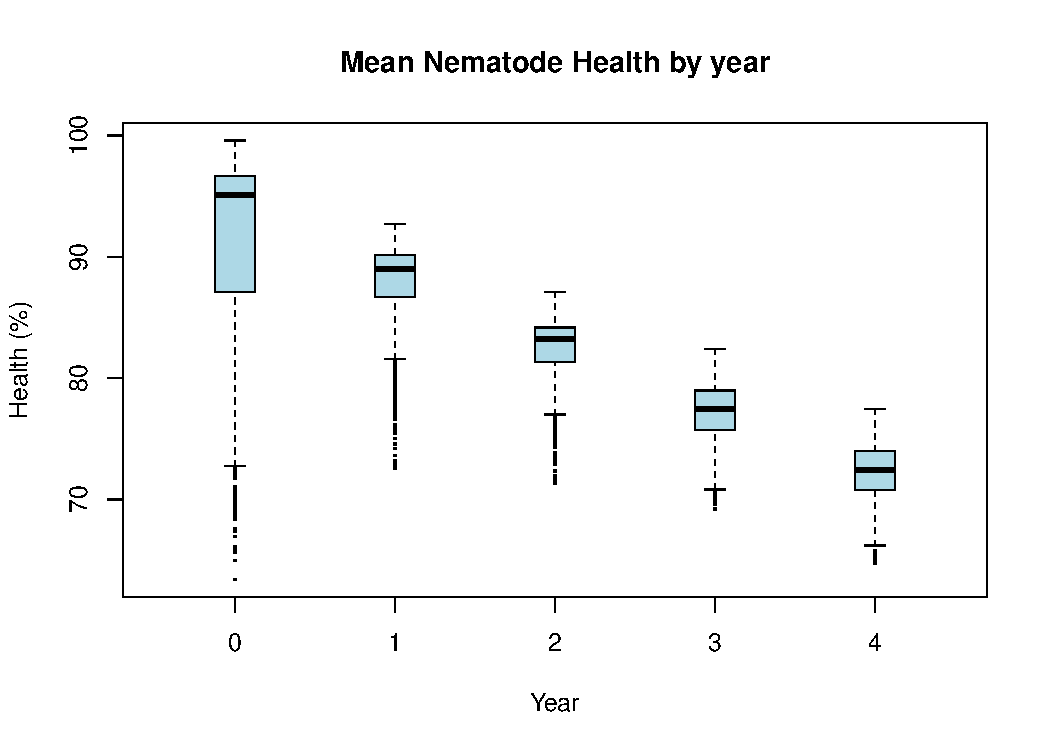
\includegraphics{figure/box-more2} 
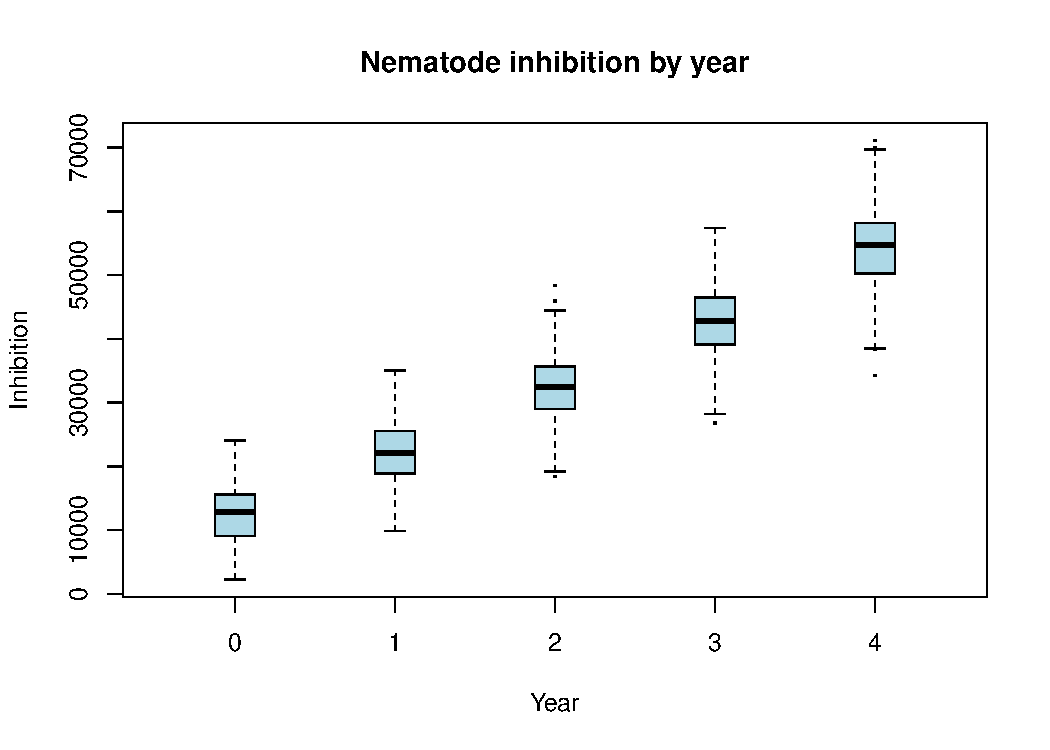
\includegraphics{figure/box-more3} 

}



\end{knitrout}

\section{Compare with Low Incidence Infection}

\begin{knitrout}
\definecolor{shadecolor}{rgb}{0.969, 0.969, 0.969}\color{fgcolor}\begin{kframe}
\begin{alltt}
lowinf <- \hlfunctioncall{dbGetQuery}(con, \hlstring{"select * from LowIncidenceInfection_dat"})
lowinf$NemDiff <- \hlfunctioncall{c}(0, \hlfunctioncall{diff}(lowinf$Nematodes))

\hlfunctioncall{ks.test}(lowinf$Nematodes, zinf_sub$Nematodes)
\end{alltt}


{\ttfamily\noindent\color{warningcolor}{\#\# Warning: p-values will be approximate in the presence of ties}}\begin{verbatim}
## 
## 	Two-sample Kolmogorov-Smirnov test
## 
## data:  lowinf$Nematodes and zinf_sub$Nematodes 
## D = 0.4964, p-value < 2.2e-16
## alternative hypothesis: two-sided
\end{verbatim}
\end{kframe}
\end{knitrout}

\begin{figure}


